\chapter{Arquitectura 4+1}

\begin{flushleft}
	La \textbf{arquitectura 4+1} es un \textbf{modelo para describir la arquitectura de sistemas de software intensivo utilizando múltiples vistas concurrentes}. Fue propuesto por Philippe Kruchten y organiza la descripción de la arquitectura en \textbf{cinco perspectivas} que responden a las preocupaciones de distintos \textit{stakeholders} (usuarios finales, desarrolladores, ingenieros, gestores, etc.).

\begin{itemize}
	\item \textbf{Lógica}: describe la estructura funcional y las principales abstracciones del sistema.
	\item \textbf{Procesos}: muestra el comportamiento en tiempo de ejecución, como concurrencia y sincronización.
	\item \textbf{Desarrollo}: representa la organización estática del software en el entorno de desarrollo.
	\item \textbf{Física}: describe la distribución del software sobre el hardware.
\end{itemize}

La \textbf{``+1''} corresponde a los \textbf{escenarios o casos de uso}, los cuales permiten ilustrar interacciones típicas del sistema y sirven para validar y relacionar las cuatro vistas principales.

En resumen, la arquitectura 4+1 es un \textbf{enfoque basado en vistas} que facilita documentar y comunicar la arquitectura de un sistema desde distintos puntos de vista relevantes para los interesados.
\end{flushleft}


	\begin{flushleft}
	\section{Vista de escenarios}

		La \textbf{vista de escenarios} (también conocida como \textit{vista +1} o \textit{vista de casos de uso}) es la quinta perspectiva del modelo de arquitectura 4+1. Esta vista no presenta una estructura estática por sí misma, sino que utiliza un conjunto de \textbf{casos de uso o escenarios representativos} para mostrar cómo los elementos definidos en las cuatro vistas principales (lógica, de procesos, de desarrollo y física) \textbf{interaccionan para satisfacer los requisitos del sistema}. Los escenarios describen secuencias de interacciones entre objetos y procesos, y sirven para:
		
		\begin{itemize}
			\item \textbf{Identificar y descubrir elementos arquitectónicos} durante el diseño.  
			\item \textbf{Validar e ilustrar} el diseño de la arquitectura una vez que está completo.  
			\item \textbf{Proveer narrativas concretas} que integran las otras vistas y facilitan la comunicación con los interesados.  
		\end{itemize}
		
		En esencia, la vista de escenarios actúa como \textbf{unificador y verificador} de las demás vistas del modelo 4+1, mostrando de forma práctica cómo funciona el sistema a través de ejemplos concretos de uso.
	\subsection{Diagrama de casos de uso}
	
	A continuación, se describen los \textbf{escenarios de la vista +1 (vista de escenarios)} basándose en la \textbf{Tabla 3.1 (Requerimientos Funcionales, pág. 39)} y en los \textbf{Requerimientos No Funcionales (pág. 41)}.
	
	\begin{figure}[H]
		\centering
		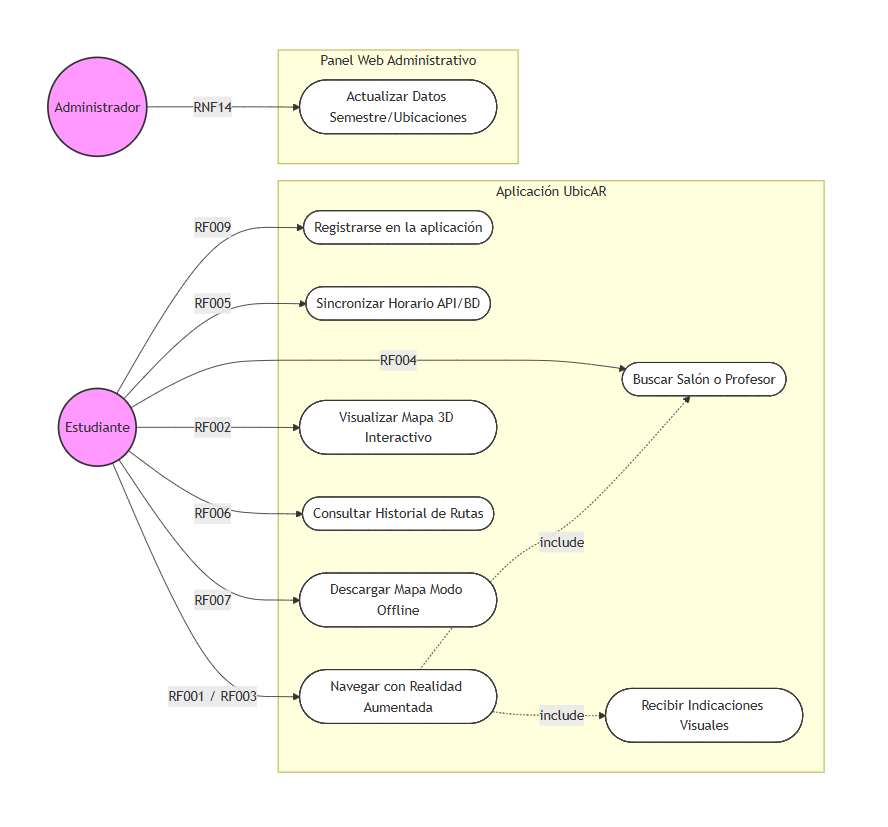
\includegraphics[width=0.95\textwidth]{imagenes/vista-escenarios.png}
		\caption{Vista de escenarios de la aplicación UbicAR}
		\label{fig:vista-escenarios}
	\end{figure}
	
	\newpage
	
	\subsection*{Actor: Estudiante}
	
	El \textbf{estudiante} es el usuario principal de la aplicación dentro de la UPIICSA. Sus escenarios clave son los siguientes:
	
	\begin{itemize}
		\item \textbf{Navegar con Realidad Aumentada (RF001, RF003, RF008):}  
		Es el escenario principal (\textit{Core}) del sistema. El estudiante selecciona un destino dentro del campus y la aplicación utiliza la cámara del dispositivo para detectar su ubicación en interiores, superponiendo flechas direccionales y elementos visuales en el entorno real para guiarlo hasta su destino.
		
		\item \textbf{Sincronizar Horario (RF005):}  
		El estudiante conecta la aplicación con su horario escolar. A partir de esta información, el sistema puede sugerir automáticamente a qué salón debe dirigirse según la hora y el día, reduciendo la necesidad de búsquedas manuales.
		
		\item \textbf{Buscar Salón o Profesor (RF004):}  
		El usuario ingresa manualmente el nombre de un profesor o el número de un aula, y el sistema calcula y muestra la ruta correspondiente dentro del campus.
		
		\item \textbf{Modo Offline (RF007):}  
		El estudiante descarga previamente los mapas y datos del semestre, lo que le permite utilizar la navegación y visualización del campus sin necesidad de conexión a internet.
		
		\item \textbf{Visualizar Mapa 3D (RF002):}  
		Como alternativa a la navegación con realidad aumentada, el estudiante puede consultar un mapa tridimensional del edificio, donde se muestra su posición y las rutas disponibles.
	\end{itemize}
	
	\subsection*{Actor: Administrador (Personal no técnico)}
	
	Este actor se identifica a partir del requerimiento \textbf{RNF14 (Actualización de Datos, pág. 41)}.
	
	\begin{itemize}
		\item \textbf{Actualizar Datos:}  
		Al inicio de cada semestre, los horarios, la ubicación de salones y los cubículos de los profesores pueden cambiar. El administrador utiliza un \textbf{panel web administrativo} para actualizar esta información sin requerir conocimientos técnicos ni la publicación de una nueva versión de la aplicación en las tiendas.
	\end{itemize}
	
	\subsection*{Justificación Arquitectónica (Modelo 4+1)}
	
	De acuerdo con lo establecido en las páginas 36 y 42 del documento, la \textbf{vista de escenarios} cumple las siguientes funciones:
	
	\begin{itemize}
		\item \textbf{Guiar el diseño de la arquitectura:}  
		Escenarios centrales como la \textit{Navegación con Realidad Aumentada} implican la necesidad de componentes de \textbf{visión por computadora} y frameworks de AR (por ejemplo, Vuforia o AR Foundation), los cuales se reflejan directamente en la \textbf{Vista Lógica}.
		
		\item \textbf{Validar la arquitectura propuesta:}  
		La correcta ejecución de escenarios como \textit{Sincronizar Horario} y \textit{Actualizar Datos} confirma que la \textbf{Vista de Datos} y la comunicación con el \textbf{Backend} (RNF10) están adecuadamente definidas y soportan los requerimientos del sistema.
	\end{itemize}
	

\end{flushleft}
	\begin{flushleft}
	\section{Vista de procesos}

		La \textbf{vista de procesos} en el modelo de arquitectura \textbf{4+1} describe los \textbf{aspectos dinámicos del sistema en tiempo de ejecución}. Se enfoca en cómo se organizan y coordinan los procesos e hilos, la comunicación entre ellos y el manejo de la concurrencia, sincronización, rendimiento y escalabilidad, con el fin de satisfacer los requerimientos no funcionales del sistema.
		
		Describe cómo se organizan los procesos, cómo se comunican entre sí y cómo se comporta el sistema bajo condiciones como concurrencia, distribución, rendimiento o escalabilidad. Es especialmente útil para analizar requisitos no funcionales relacionados con el comportamiento durante la ejecución del sistema y suele representarse con diagramas UML como diagramas de actividad o de secuencia.
		
		\subsection{Diagrama de Secuencia}
		
		Basado en los \textbf{Requerimientos Funcionales} (Capítulo 3, pág. 39) y en el flujo de trabajo descrito en el \textbf{Marco Teórico} (Figura 2.2, pág. 15), la Figura \ref{fig:vista-procesos} presenta el \textbf{diagrama de secuencia} que representa el escenario principal: \textit{``El estudiante consulta su horario y navega hacia su salón usando Realidad Aumentada''}.  
		
		Este diagrama detalla la interacción entre el usuario, la interfaz de la aplicación, el motor de realidad aumentada y el backend de datos.
		
		\begin{figure}[H]
			\centering
			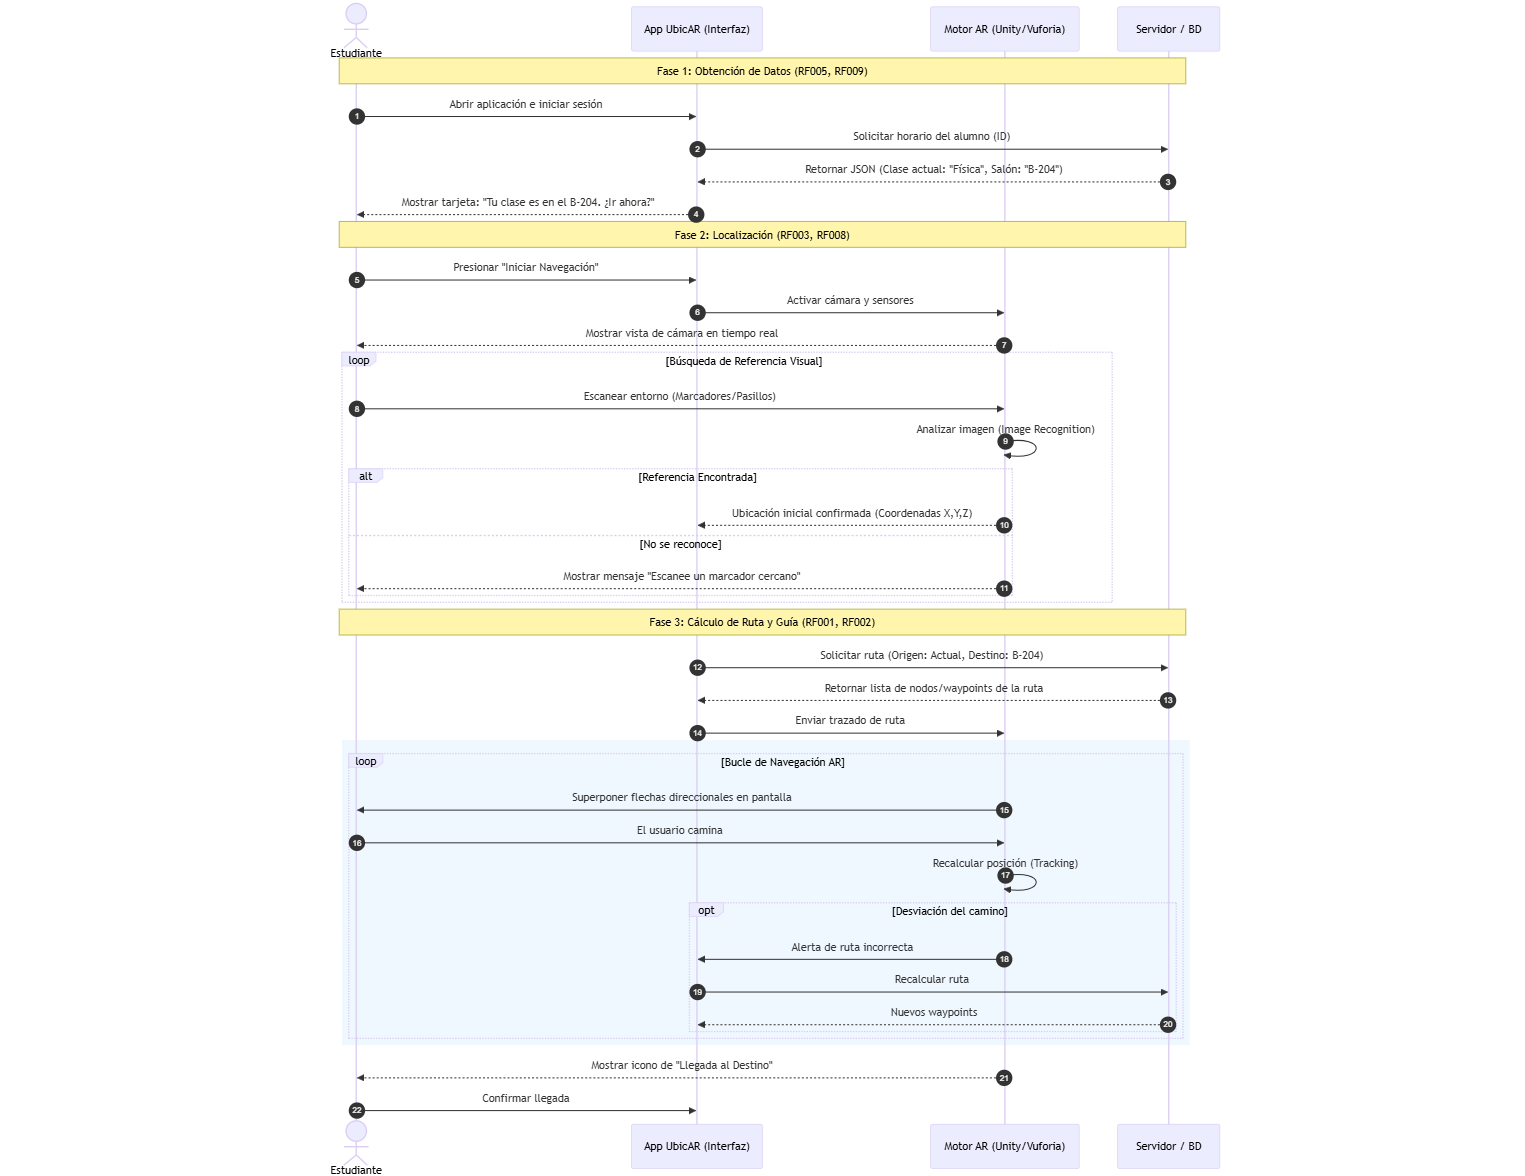
\includegraphics[width=0.95\textwidth]{imagenes/vista-procesos.png}
			\caption{Diagrama de secuencia del escenario principal de navegación con Realidad Aumentada}
			\label{fig:vista-procesos}
		\end{figure}
		
		\subsection*{Participantes}
		
		\begin{itemize}
			\item \textbf{Estudiante:} Usuario final que interactúa con la aplicación.
			\item \textbf{App UbicAR:} Capa de presentación y lógica de negocio ejecutada en el dispositivo móvil, desarrollada en \textit{Unity} con \textit{C\#}.
			\item \textbf{Motor AR:} Componente técnico responsable del procesamiento de visión por computadora y la detección del entorno, implementado mediante \textit{Vuforia} (según págs. 11 y 17).
			\item \textbf{Backend:} Servicio de datos o API que almacena la información de edificios, aulas y horarios.
		\end{itemize}
		
		\subsection*{Fases del Flujo}
		
		\begin{itemize}
			\item \textbf{Fase 1 – Obtención de Datos:}  
			Corresponde al requerimiento \textbf{RF005 (Sincronización de Horario)}. El sistema consulta el backend para obtener el horario del estudiante, permitiendo que la aplicación conozca el destino antes de que el usuario realice una búsqueda manual.
			
			\item \textbf{Fase 2 – Localización:}  
			Asociada a los requerimientos \textbf{RF003 (Detección de Ubicación)} y \textbf{RF008}. En esta fase se utiliza la tecnología de \textbf{Vuforia} para reconocer la posición del usuario dentro del edificio mediante marcadores visuales o características del entorno.
			
			\item \textbf{Fase 3 – Navegación:}  
			Representa el núcleo del sistema y cubre el requerimiento \textbf{RF001 (Guía Visual)}. Se muestra un bucle continuo en el que el usuario avanza físicamente mientras el sistema recalcula su posición y actualiza las flechas direccionales en tiempo real hasta alcanzar el destino.
		\end{itemize}
		
\end{flushleft}



	\section{Vista lógica}

La vista lógica de UbicAR sigue un patrón de arquitectura en capas para garantizar la escalabilidad y el mantenimiento. Se divide principalmente en tres niveles:

\begin{itemize}
    \item \textbf{Capa de Aplicación(Frontend):} Contiene la lógica de la interfaz de usuario, el motor de renderizado de Realidad Aumentada y la gestión de sensores del dispositivo móvil.
    
    \item \textbf{Capa de Servicio(API/Backend):} Actúa como intermediario, procesando las solicitudes de rutas y filtrando la información de profesores y salones antes de enviarla al móvil.

    \item \textbf{Capa de Persistencia:} Encargada de la comunicación con la base de datos SQL Server para recuperar horarios y coordenadas geográficas.
\end{itemize}

\begin{figure}[H]
		\centering
		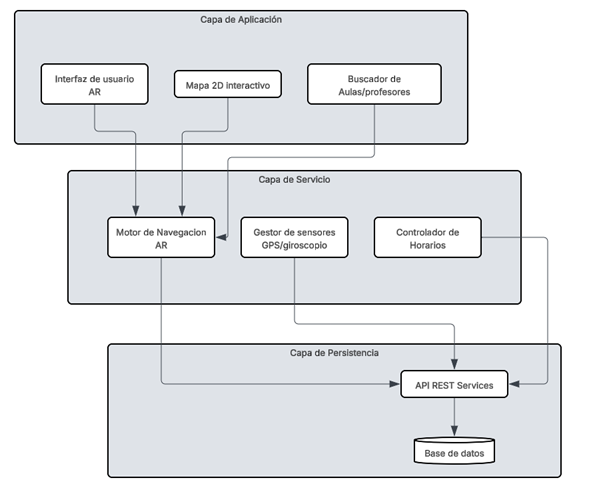
\includegraphics[width=0.95\textwidth]{imagenes/vista-logica.png}
		\caption{Diagrama de Capas de la Vista Lógica}
		\label{fig:vista-logica}
	\end{figure}

	\section{Vista física}

La vista física describe la infraestructura tecnológica sobre la cual se despliega la solución UbicAR. La arquitectura se distribuye en cuatro nodos principales:

\begin{itemize}
    \item \textbf{Nodo Smartphone:} Es el núcleo de la experiencia de usuario. No es solo un teléfono; el sistema utiliza la IMU (Inertial Measurement Unit) —acelerómetro y giroscopio— para mantener la estabilidad de los objetos virtuales (flechas, etiquetas) mientras el estudiante camina. La Cámara realiza el rastreo de características visuales del entorno.

    \item \textbf{infraestructura de Red:} Dado que el GPS suele perder precisión dentro de edificios (problema común en universidades), la vista física contempla los Puntos de Acceso Wi-Fi para ayudar a la triangulación de la ubicación del usuario.

    \item \textbf{Servidor de Aplicaciones:} Este nodo procesa la lógica pesada. No solo envía texto; es el encargado de servir los Assets AR (iconos de facultades, modelos 3D de flechas) al dispositivo móvil.

    \item \textbf{Servidor SQL Server:} Es el nodo de persistencia. Aquí se realizan las consultas complejas de horarios y cruces de información entre profesores y aulas.
\end{itemize}

	\input{./arquitectura4+1/secciones/despliegue}
	\input{./arquitectura4+1/secciones/datos}
